% THIS IS AN EXAMPLE DOCUMENT FOR VLDB 2012
% based on ACM SIGPROC-SP.TEX VERSION 2.7
% Modified by  Gerald Weber <gerald@cs.auckland.ac.nz>
% Removed the requirement to include *bbl file in here. (AhmetSacan, Sep2012)
% Fixed the equation on page 3 to prevent line overflow. (AhmetSacan, Sep2012)

\documentclass{vldb}
\usepackage{graphicx}
\usepackage{balance}  % for  \balance command ON LAST PAGE  (only there!)


\begin{document}

% ****************** TITLE ****************************************

\title{Survey on Re* Research}

% possible, but not really needed or used for PVLDB:
%\subtitle{[Extended Abstract]
%\titlenote{A full version of this paper is available as\textit{Author's Guide to Preparing ACM SIG Proceedings Using \LaTeX$2_\epsilon$\ and BibTeX} at \texttt{www.acm.org/eaddress.htm}}}

% ****************** AUTHORS **************************************

% You need the command \numberofauthors to handle the 'placement
% and alignment' of the authors beneath the title.
%
% For aesthetic reasons, we recommend 'three authors at a time'
% i.e. three 'name/affiliation blocks' be placed beneath the title.
%
% NOTE: You are NOT restricted in how many 'rows' of
% "name/affiliations" may appear. We just ask that you restrict
% the number of 'columns' to three.
%
% Because of the available 'opening page real-estate'
% we ask you to refrain from putting more than six authors
% (two rows with three columns) beneath the article title.
% More than six makes the first-page appear very cluttered indeed.
%
% Use the \alignauthor commands to handle the names
% and affiliations for an 'aesthetic maximum' of six authors.
% Add names, affiliations, addresses for
% the seventh etc. author(s) as the argument for the
% \additionalauthors command.
% These 'additional authors' will be output/set for you
% without further effort on your part as the last section in
% the body of your article BEFORE References or any Appendices.

\numberofauthors{2} %  in this sample file, there are a *total*
% of EIGHT authors. SIX appear on the 'first-page' (for formatting
% reasons) and the remaining two appear in the \additionalauthors section.

\author{
% You can go ahead and credit any number of authors here,
% e.g. one 'row of three' or two rows (consisting of one row of three
% and a second row of one, two or three).
%
% The command \alignauthor (no curly braces needed) should
% precede each author name, affiliation/snail-mail address and
% e-mail address. Additionally, tag each line of
% affiliation/address with \affaddr, and tag the
% e-mail address with \email.
%
% 1st. author
\alignauthor
Serhiienko Oleksii
       \affaddr{InIT Cloud Computing Lab, Zurich University of Applied Sciences}
       \affaddr{Winterthur, Switzerlande}\\
       \email{serh@zhaw.ch}
% 2nd. author
\alignauthor
Dr. Josef Spillner
       \affaddr{InIT Cloud Computing Lab, Zurich University of Applied Sciences}
       \affaddr{Winterthur, Switzerlande}\\
       \email{spio@zhaw.ch}
}
% There's nothing stopping you putting the seventh, eighth, etc.
% author on the opening page (as the 'third row') but we ask,
% for aesthetic reasons that you place these 'additional authors'
% in the \additional authors block, viz.
\additionalauthors{Additional authors: John Smith (The Th{\o}rv\"{a}ld Group, {\texttt{jsmith@affiliation.org}}), Julius P.~Kumquat
(The \raggedright{Kumquat} Consortium, {\small \texttt{jpkumquat@consortium.net}}), and Ahmet Sacan (Drexel University, {\small \texttt{ahmetdevel@gmail.com}})}
\date{30 July 1999}
% Just remember to make sure that the TOTAL number of authors
% is the number that will appear on the first page PLUS the
% number that will appear in the \additionalauthors section.


\maketitle

\begin{abstract}
-
\end{abstract}




\section{Introduction}
Computer science world and research which involves \\ computation-based experiments have complex processes and interactions of embedded and real-time systems, compilers, networking, and operating systems. Unfortunately, with growing system complexity, it is getting more difficult to get the same results and conclusions which are provided by original scientific work which is leading to decreasing quality of research. That is why research world came with Re* research concept. \emph{Re* research} refers to processes with outputs and documentation which ensure \emph{repeatable, reproducible, recomputable, reusable} or \emph{replicable} results. In the scientific community, there is increasing concern about these characteristics, as evidenced by recent reports from ACM, Dagstuhl, and other players. The goal of this work is to consolidate and structure the knowledge around Re* research as well as the reflection and reception in the scientific community, including in conference and journal and submission requirements. All these best practices will lead to general paper and research quality improving.

\subsection{Motivation}
Publications are one of the most critical and essential foundations of academic life. At the same time Jan Vitek\cite{DBLP:conf/emsoft/VitekK11} tells that computational disciplines have much more advantages in comparison with other fields of science since in most cases conferences plays the role of a filter for selecting the best scientific works. Unfortunately, due to the short publication time and the one-stage process of reviewing papers, the conferences had a profound impact on how the procedures in research are now being carried out. To remain competitive due to time constraints and unregulated standards of reproducibility of scientific works, most researchers had to decrease the level of research quality and not spend the majority of time to prepare, provide and publish code and documentation. Also, due to the increasing complexity of scientific experiments with the rapid growth of technical progress, as well as the fact that the main criteria for most conferences in the evaluation of scientific papers are the level of novelty - most Re*research concepts are increasingly ignored during publication writing.\par
In our days for computational-based experiments, all the processes that are performed while writing scientific work can be characterized as follows: \par
The researcher identifies the problem that has not yet been solved or solved non-effectively. In the future, the software is written, which conducts evaluation and tests of the task/problem. When programming is complete,  initiated the process of preparation of the initial data that will be processed by the software. When the result data is ready, it is analyzed by researcher and proofs hypothesis or creates brand new ideas based on the data. This workflow is shown in the picture: \ref{fig:workflow} \par
\begin{figure}[h!]
  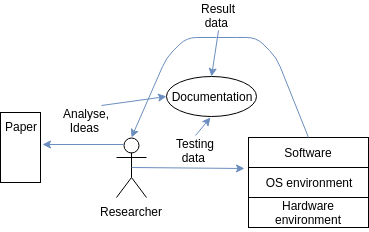
\includegraphics[scale=0.6]{fig/reresearch.png}
  \caption{Research workflow}
  \label{fig:workflow}
\end{figure}

\par By Jan Vitek\cite{DBLP:conf/emsoft/VitekK11} the essence of the scientific process in computer systems consists of:
\begin{itemize}
    \item Identifying a problem and positing a hypothesis or model.
    \item Engineering a concrete implementation.
    \item Designing and conducting an experimental evaluation.
\end{itemize} \par

\subsection{Problem statement}
Experiments which includes computations, commonly represent complex ideas, and it is necessary to carry out a lot of tests on various of hardware and software platforms with several implementations. Typically, this is beyond the limitations caused by the amount of time and paper size. As a result, documents and scientific works that can be useful to the academic community are published without sufficient documentation, mention of restrictions and adequate instructions to reproduce the experiment and results. \par
Reasons above led to the fact that the academic community came to the idea of Re* research. Re* research refers to processes with outputs and documentation which ensure repeatable, reproducible, recomputable, reusable or replicable results. Instead, by Collberg\cite{DBLP:journals/cacm/CollbergP16} the symptoms of the current state of practice include:
\begin{itemize}
    \item Unrepeatable results
    \item Unreproduced results 
    \item Measuring the wrong thing 
    \item Meaninglessly measuring the right thing. 
\end{itemize} \par
Jan Vitek\cite{DBLP:conf/emsoft/VitekK11} defines more factors apart from pressure which are leading to bad quality from Re* research point of view:
\begin{itemize}
    \item Lack of benchmarks
    \item Lack of experimental methodology
    \item Lack of understanding of statistical methods
\end{itemize}
Tomas Kalibera in his work\cite{DBLP:conf/popl/Vitek15} "Repeatability, reproducibility in computer systems research" defines 7 "Deadly sins" in research which are making end results much useless :
\begin{itemize}
    \item \textbf{"Unclear experimental goals."} First of all, it is necessary to formulate the purpose of the experiment and what kind of results and conclusions are expected in the end. Without clearly posed questions, the experiment has not much sense.
    \item \textbf{"Implicit assumptions or experimental methodology."}. The documentation should have full information about the experimental setup and methodology that were used in conducting the experiment.
    \item \textbf{"Proprietary benchmarks and data sets."} For many researchers, as well as for industry, the availability of benchmarks and data sets used in the experiment could be a key point.
    \item \textbf{"Weak statistical analysis."} Even at high-level conferences like PLDI’11 \cite{DBLP:conf/pldi/2011}, most of the works ( 39 of 42) did not mention about the division in a time of executed experiments.
    \item \textbf{"Measuring the wrong thing/right thing meaninglessly."} Often a situation occurs when complex and non-trivial experiments involve incorrect connections between various factors.
    \item \textbf{"Lack of a proper baseline."} Many researchers while writing a paper use own implemented baseline with differing levels of optimization. Therefore, it is essential at the beginning of the experiment to establish a reliable and credible baseline.
    \item \textbf{"Unrepresentative workloads."} One of the biggest dangers of writing a regular paper is the wrong load on the computer system. Processes that performs in parallel with the conducted experiment can have a fundamentally affect on the result and could not be reproduced in the future.
\end{itemize}
\subsection{Methodology}
To write this survey paper, scientific papers, articles, and posts were analyzed. Most of the time, data sources were found and taken from both DBLP\cite{dblp} and Google Scholar\cite{google}. In total, 75 scientific papers were analyzed, and for each of the characteristics of the Re* research, 3-5 papers were selected. The analysis of the scientific material was carried out to compile a general picture and the relationship between the characteristics given above, each of which is central in a variety of scientific publications. All the selected scientific works were abstracted on the problem they cover, and year of publishing. The figure\ref{fig:figure1} shows a graph with the number of publications where certain characteristic was a central problem. For making this analysis, the full list of papers was used (see Appendix) and simple Python code which together with initial data can be found on GitHub\cite{gith}. 
\begin{figure}[h!]
\hspace*{-1.5cm}  
  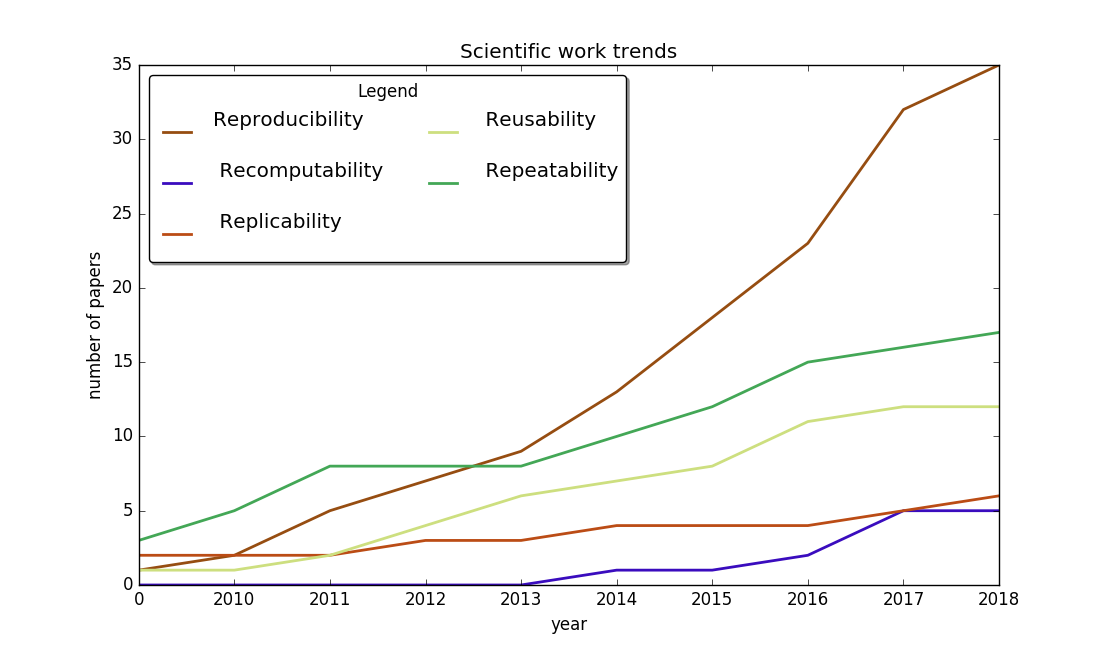
\includegraphics[scale=0.40]{fig/figure1.png}
  \caption{Paper analysis}
  \label{fig:figure1}
\end{figure} \par
The primary requirements were the quality of the paper, documents with later dates had a privilege and, of course, papers were chosen which determined the research characteristics of Re *research as a central topic. From the analyzed articles, the most prominent efforts were made to extract definitions, features, current solutions and generalize them to give a clear idea of these topics separately and to create a "general view" of the study. The "general view" implied a clear division and commonalities between each part of the Re* study. As a result, the goal was also to make a set of simple requirements that will help make scientific work reproducible/repeatable/recomputable/reusable/replicable.


\section{}{Re* research characteristics}
\subsection{Repeatability}
The repetition by Tomas Kalibera\cite{DBLP:conf/popl/Vitek15} definition is "the possibility of repeating the same experiment, simulation or scientific method in the same system and way and obtaining the same result." This requirement applies more to researchers to ensure stable results, but is also necessary for the scientific community in particular. Having the opportunity to repeat the result leads to new ideas. When the results are repetitive, it makes it easier for systems research. This characteristic is beneficial for scientific reviewers since those works/results that are repetitive and provide a code or web interface in the public domain can be tested for reliability. And also to evaluate the proposed method, the change in input data can be used. Especially this applies to those works for which no special hardware or software infrastructure is required. \par
Another author Collberg\cite{DBLP:journals/cacm/CollbergP16} defines the repeated study as " if it is possible to re-run the researchers experiment using the same method in the same environment and obtain the same results." In his opinion, it is necessary to keep results repeatable that reviewers, colleagues and other scientists could evaluate the outcome and methodology by full and accurate evidence. With this approach, a lot of repetitive work will be avoided; the researchers rely on the result and scientific progress will advance. \par
In this work, repeatability can be defined as an ability of scientific work to be repeated the various number of times and receive the entirely the same result of each experiment. The researcher needs to provide full information about his experimental set-up, software, codebase and initial datasets with instructions how to run them. This workflow is shown in the picture \ref{fig:repeatability}. \par
\begin{figure}[h!]
  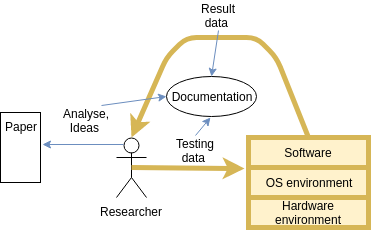
\includegraphics[scale=0.6]{fig/repeatability.png}
  \caption{Repeatability}
  \label{fig:repeatability}
\end{figure}
\subsubsection{Current state of art}
The National Science Foundation Grant Proposal Guide\cite{nfsgp} says, “Investigators and grantees are encouraged to share software and inventions created under the grant or otherwise make them or their products widely available and usable.” 
Typically, papers from industry have low repeatability because most of the code is under a private license, at the same time academic works, because they use open-source code, have a higher degree of repeatability.
\subsubsection{Recommendations}
\begin{itemize}
    \item One of the most widely used practices to ensure scientific work is repeatable is the packaging of all source data, code, operating system, and third-party software into a \textbf{virtual image}. This practice will allow the project to be run by any researcher and solve problems with the versioning. The more it leads to own issues and limitations that need to be resolved. Like how to solve the problem with the launching of a virtual image that may have had an outdated operating system or applications that have identified the security vulnerabilities and at the moment they are not patched, and still, results might be different because of hardware setup, etc.
    \item \textbf{Fund repeatability engineering}. Special agencies should encourage researchers to request additional funds for “repeatability engineering,” including hiring programming staff to document and maintain code, do release management, and assist other research groups wanting to repeat published experiments. In the same way funding agencies conduct financial audits to ensure costs claimed by grantees are allowed, they should also conduct random audits to ensure research artifacts are shared by what was promised in the grant application
    \item \textbf{Require sharing contract}. Publishers of conference proceedings and journals should require every article include a sharing contract specifying the level of repeatability to which its authors will commit. While the first point will have the effect of shifting some funding from pure research to engineering and oversight, both are important because they ensure research results continue to benefit the academic community— and the public funding it—past the project end date. 
    \item \textbf{Sharing contracts}. The sharing contract should be provided by the authors when a paper is submitted for publication (allowing reviewers to consider the expected level of repeatability of the work), as well as in the published version (allowing readers to locate research artifacts). The contract commits the author to make certain available resources that were used in the research leading up to the paper and committing the reader/reviewer to take these resources into account when evaluating the contributions made by the paper
\end{itemize}
\subsection{Reproducibility}
Many research departments recently have been increasingly worried by the reproducibility of scientific papers, especially in computation-based experiments, where computers and computations are the central part of the experiment. To ensure performance is necessary to publish all the computational tools, documentation, datasets and benchmarks that were used by the researchers for this experiment. For any researcher who would like to reproduce results and experiments open source code, documentation, datasets should be available. This movement in the scientific world has a de facto title "Reproducible research"\cite{DBLP:journals/jetai/Drummond18}. \par
In the work of Tomas Kalibera\cite{DBLP:conf/popl/Vitek15}, reproducibility is defined as: "Independent confirmation of a scientific hypothesis through reproduction by an independent researcher/lab is at the core of the scientific method." Reproduction of scientific work should be done by independent researchers after publishing the paper with available datasets, code, experimental setup, etc. Required data can also be requested from the author. It is also possible to say that in the case of error or deception of work reproducibility is better to use compared to repeatability since it provides a higher level of abstraction.\par
Comparing repeatability and reproducibility, another author Colberg\cite{DBLP:journals/cacm/CollbergP16} notes that reproducibility does not require an identical experimental setup with the same hardware. Instead, it is an independent confirmation of the scientific hypothesis/results that are performed after the publication by other research units conducting the same experiments with the same or similar data periodically changing them that come to the similar or the same conclusions. It can be concluded that: Repeatability and reproducibility are characteristics of the scientific workflow that is necessary to prevent the proliferation of erroneous results. \par
In this work, reproducibility can be defined as an ability of scientific work to be reproduced by any other research group not depending on hardware requirements. Compared to repeatability, results should not be identical but rather conclusions and data trends should be confirmed. A researcher needs to provide full information about codebase and initial datasets with instructions how to run them. Although an alternative solution that also confirms the conclusions can be considered reproducible. This workflow is shown in the picture \ref{fig:reproducability}.\par
\begin{figure}[h!]
  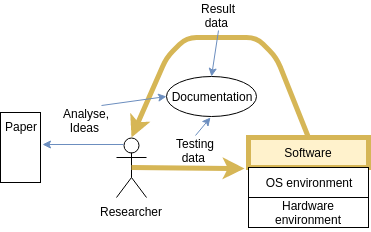
\includegraphics[scale=0.6]{fig/reproducibility.png}
  \caption{Reproducibility}
  \label{fig:reproducability}
\end{figure}
\subsubsection{Current state of art}
Since the problem of the reproducibility of scientific works is not new, many scientific journals like PLOS and  Nature Methods with some governmental institutions such as NIH require authors to provide all the data obtained during the experiments. Data include documented steps of experiments and intermediate results, in order so that interested parties have access to this information, and there is an opportunity to promote similar research. Often, studies that reproduce already existing hypotheses are also published in journals whether they confirm whether or not the results of the original study. In the world of computer science, unfortunately, this does not happen, although there have been numerous attempts at the Reproducing research planet\cite{rrp}, and the Evaluation of Collaboratory\cite{evcol}. The reproducible research planet is a website for scientists who must store research data including data sets, code, documentation, experimental setup, etc. There have been attempts to make this website part of a standard research process in several articles and journals. In turn, the authors thereby increased their chance to be cited and reproducibility in general. The Evaluate Collaboratory is in addition to organizing workshops on experimental evaluation of software and computer systems, initiated a petition to program committee chairs of conferences and workshops that called for acceptance of reproduction studies as first-class publications.
\subsubsection{Recommendations}
\begin{itemize}
    \item \textbf{Develop open source benchmarks}. Required benchmarks, well documented, open source and carefully evaluated benchmarks should be fully accepted as first-class contributions for publications at leading conferences and journals and should be supported.
    \item \textbf{Codify best practice documentation, methodologies and reporting standards}. It is necessary to harmonize the minimum standards for documenting experiments and reporting. This can be done through community efforts and target working groups. It is also required to understand the factors that affect the measurable properties of computer systems, and better understand their statistical properties.
    \item \textbf{Require repeatability of published results}. Repeatability should be part of the publication review process. Based on the document and additional material on the experiments (documentation, configuration, source code, input sets, scripts), reviewers should make sure that the experiments are repeatable.
\end{itemize}
\subsection{Recomputability}
In work "The Recomputation Manifesto"\cite{DBLP:journals/corr/abs-1304-3674} Gent indicates that in the scientific development, replication is of great importance, but usually, in the computer science world, replication does not take much attention and researchers do not repeat the same experiment over and over again. And those experiments that are rarely implemented do this in full. The manifesto proposes to make the source code more accessible, although this is a small step. Usually, even when the source code can be launched this does not mean that the experiment can be repeated. In this paper, it is proposed that the discipline of computer science include the replication of experiments as a standard practice and also that tools and repositories are available..\par
Some of the authors\cite{DBLP:conf/psb/KaushikISTDK17} define recomputability the same as reproducibility as the ability to achieve the same results on the same data regardless of the computing environment or when the analysis is performed.\par
In his paper\cite{DBLP:conf/ucc/WehrleLVR14}, Wehrle notes that research is currently associated with highly specialized software and complex data processing workflows. While technology accelerates scientific progress, this acceleration also risks the sustainability of progress. Since almost every piece of information is created, transmitted and stored digitally, and the information is not necessarily associated with single, easily identifiable digital objects, but can be embedded in complex environments and processes, which allows to check, replicate and reuse data and accompanying methods not guaranteed, especially in the long run.\par
Matthias Kricke\cite{DBLP:journals/dbsk/KrickeGS17} provides one of the most accurate definitions of replication, this "ability to recompile results from raw data at any time" is essential for these studies to ensure data stability and selectively include new data in the already supplied data product. The competence of these products allows the client to restore earlier versions of data, reports and analysis results to compare them with new ones.\par
In this work, recomputability can be defined as an ability of scientific work to be recomputed any point in time with any data and by anyone who would like to do it. A researcher needs to provide full information about codebase and make it publicly available. Compare to reproducibility and repeatability the goal is not to get the same results or conclusions, but instead, other people can reuse codebase for any purposes. This workflow is shown in a picture \ref{fig:recomputability}.\par
\begin{figure}[h!]
  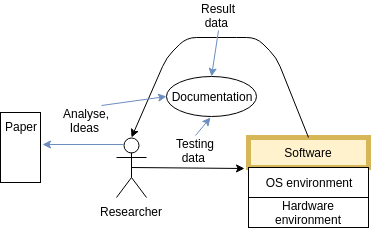
\includegraphics[scale=0.6]{fig/recomputability.png}
  \caption{Recomputability\cite{gith}}
  \label{fig:recomputability}
\end{figure}
\subsubsection{Current state of art}
Minimum information standards for recomputable experiments have been discussed and publically available for some years (e.g.,  MIAME\cite{MIAME}, MIABi\cite{MIABi}), although much recent discussion on the practical implementations of recomputability frequently takes place on the Internet and in blogs rather than in peer-reviewed literature\cite{ivory}\cite{recomputation}\cite{bioinformaticszen}. 
\subsubsection{Recommendations}
\begin{itemize}
    \item Each publication presenting computational results should be aimed at creating a "virtual reference environment" accompanying the publication. This reference environment should be the minimum implementation of the software stack needed to reproduce some or all of the computational part of the results. For a desktop tool, this will be the operating system, libraries, tools, and data. By downloading this image and placing it on a virtual machine monitor, such as VMWare \cite{vmware} or VirtualBox \cite{virtualbox}, readers and reviewers can immediately reproduce and examine the results with minimal setup effort. Many researchers now also have access to institutional or national "cloud" environments, and a virtual reference environment can easily be applied to one of them.
    \item Using open and free software, such a reference medium is now technically simple for production and distribution; it does not require specialized knowledge in the field of software development or system administration beyond the skills set of a typical bioinformatics researcher. If the result is operating systems and tools with open source code or software, there are step-by-step tools for creating a snapshot of the working environment (for example, Ubuntu Builder \cite{launchpad} or Relinux).
    \item Using already existing tools like Popper\cite{DBLP:conf/infocom/JimenezAALMMR17}, which goal is to implement executable papers in today's cloud-computing world by treating an article as an open source software (OSS) project. Popper is realized in the form of a convention for systematically implementing the different stages of the experimentation process following a DevOps approach.
\end{itemize}
\subsection{Reusability}
One of the complete works on the scientific works reusability belongs to Costantino Thanos\cite{DBLP:journals/publications/Thanos17} in his the term re-use of data means the ease of using data collected for one purpose, to study a new problem. This term implies re-use of separate data sets in the context of different contexts. Re-use of data becomes a unique feature of modern scientific practice, as it allows for the re-examination of evidence, reproduction, and verification of results, minimizing duplication of effort and relying on the work of others.\par 
In another paper, Gabriel Fils\cite{DBLP:journals/corr/ThatFYM17} say that the minimal use case for sharing a computational experiment (in the form of a joint research object) involves repeating its initial implementation and verifying its results. However, to use its potential, it must support modified reuse. The objective of research should be created and stored not as a simple aggregate of digital content, but in an efficiently computable form: as a reusable object.\par
In this work, reusability can be defined as an ability of scientific work to be reused any point of time with any data and by anyone who would like to do it and ultimately everything should be documented starting from the progress, small conclusions, ideas, methods, and benchmarks choice. A researcher needs to provide full information about codebase, datasets, and documentation. The main idea that other researcher can reuse the data to make brand new conclusions/papers. This workflow is shown in the picture \ref{fig:reusability}.\par
\begin{figure}[h!]
  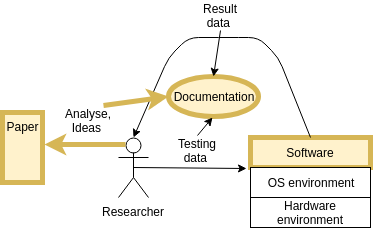
\includegraphics[scale=0.6]{fig/reusability.png}
  \caption{Reusability}
  \label{fig:reusability}
\end{figure}
\subsubsection{Current state of art}
The ability to reuse data can be efficiently implemented within Open Science since the ultimate goal of Open Science is to make research data public and reusable. The European Commission is moving decisively towards the implementation of the "Open Science" concept in Europe: in 2015, the European Commission called on all member states of the European Union to ensure that states publish public research results to improve science and strengthen their knowledge-based\cite{reus1}. The recent "Amsterdam Call to Action on Open Sciences" advocates "full open access for all scientific publications" and endorses an environment in which data sharing and management are the default method for all publicly funded research. This document was prepared as an open scientific conference organized by the Dutch Presidency of the Council of the European Union (April 4-5, 2016) \cite{reus2}. Another initiative of the European Commission, which is worth mentioning, is the publication of the FAIR Data Management Guide in Horizon 2020, that is, a set of guidelines for creating data accessible, accessible, compatible and reusable \cite{reus3}. The same as SNSF in "FAIR data principles"\cite{snsf} defines a range of qualities a published dataset should have in order to be Findable, Accessible, Interoperable and Reusable.
Code, data, scenarios and the results of a temporary experiment - provide the means for sharing knowledge about computational analyses.
\subsubsection{Recommendations}
There are plenty of practices which can be applied to make proper implementation of the Data Publication procedures and, thus, to overcome the impediments to data reuse. Thanos\cite{DBLP:journals/publications/Thanos17} defines most important recommendations:
\begin{itemize}
    \item \textbf{(Meta) Data Modeling.} In order to facilitate data understandability, it is necessary to define and develop formal models that adequately describe:
    \begin{itemize}
        \item data representation needs of a given scientific discipline;
        \item data provenance information;
        \item data contextual information;
        \item data uncertainty;
        \item data quality information.
    \end{itemize}
    All this information is collectively called metadata information. If scientists need to reuse data collected by others, then the data must be carefully documented. Metadata is descriptive information about the data that explains the measured attributes, their names, units, accuracy, accuracy, a location of the data and, ideally, much more. Recently, a mechanism was proposed, a data document capable of improving the understanding of data and, therefore, the reuse of data. A data document can be defined as a scientific publication of a metadata document with a search capability describing a specific on-line available dataset or a group of datasets published by standard academic methods\cite{Chavan2011}.
    \item \textbf{Domain-Specific Ontologies Ontologies.} A key technology that allows a wide range of data transmission services\cite{DBLP:journals/tods/BienvenuCLW14}. The increasing availability of data has shifted focus from closed applications with relatively low data levels, to mechanisms and applications for searching, integrating and using the vast amounts of data that are now available. Ontologies provide a semantic basis that allows you to reuse research data\cite{Gruber:1995:TPD:219666.219701}\cite{DBLP:journals/jods/PoggiLCGLR08}.
    \item \textbf{Data Discovering.} Under the discovery of data, meaning the ability to quickly and accurately identify and find data that supports research requirements. The process of detecting data existing in the data collection/database is supported by a search and query function that uses the capabilities of registering and citing data; and metadata descriptions contained in categorization/classification schemes, data dictionaries, and metadata registries.
    \item \textbf{Data Exchangeability.} By data exchange, we mean the ability of two objects, that is, the author of data and the data user, to exchange meaningful data sets. Data exchange is a prerequisite for the reuse of data. During the data exchange process, especially when data moves between scientific disciplines, it is necessary to solve three types of "heterogeneity".
    \item \textbf{Linking Data to Publications.} In science with a predominance of data, scientific communication undergoes significant changes. Modern scientific communication should support the practice of providing a link to data in the same way that researchers usually provide a bibliographic reference to printed resources. The need for quoting data is beginning to be recognized as one of the critical practices underlying the recognition of data as primary research products and not as a by-product of research
\end{itemize}
\subsection{Replicability}
The term replicability is not defined in computer science, and most of the time it refers to reproducibility. But for example in psychological scientific research Fournier\cite{Four} explains that the study should give the same results if they are repeated precisely. The replicability can be increased by an in-depth review of other similar experiments and exclude variables that you might not have thought of. \par
At the same time, Sinha\cite{For} gives a different definition that replicability uses the same methods, but with different themes and experimenters,  can also be reproduced someone else's work or results to establish its validity. For example, if someone executes experiment A and reaches conclusion B, and if someone does the same experiment A and come to a C output that is different from B, then it will not replicate because the results will not be reproduced. \par
in the end, Fehr\cite{DBLP:journals/corr/FehrHHS16} gives quite a precise definition of replicability of the attribute describes the possibility of repeating experiments based on calculations and obtaining the same results. Sometimes this is an equivalent term. For replication, required documentation is required on how to run the software to get replicated results. Replicability, in turn, is the primary requirement of reliable software, as well as its results, as it demonstrates the absolute stability of the procedure against statistical influences and observer bias. Also, screening can serve as a benchmark against which new methods can be compared, as indicated in. \par
In this work, replicability can be defined as an ability of scientific work to be replicated by anyone. A researcher needs to provide detailed information and documentation on experiment workflow, codebase wich documentation. The main idea that other researcher can get the same conclusions. This workflow is shown in picture \ref{fig:replicability}.\par
\begin{figure}[h!]
  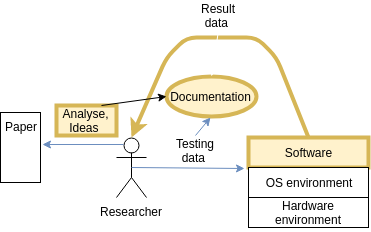
\includegraphics[scale=0.6]{fig/replicability.png}
  \caption{Replicability}
  \label{fig:replicability}
\end{figure}
\subsubsection{Current state of art}
Concerns about reproducibility are confirmed by the observation that replication studies are rare and in some areas become less frequent with time. Various authors have established links between the rarity of replicas and the importance attached to innovation and original research, or to the perception that replications are not published in journals. The Nature study showed that a minority of researchers even attempted to publish replication, although, on a positive note, 24\% published successful replication, and 13\% published a refusal to replicate the result. This is balanced approximately by the equivalent number (10\%) of respondents who reported that they could not issue the error message\cite{DBLP:conf/kolicalling/AhadiHIKP16}
\subsubsection{Recommendations}
\begin{itemize}
    \item Basic documentation. A fundamental requirement for replicability is the abbreviated documentation, which includes instructions on how to generate an executable binary program in the case of a compiled language and a description of how to run the program to obtain replicated results. This documentation is crucial for the replication of the experiment because it determines the technical implementation and provides a possible repetition of the experiment. Often numerically calculated results are further processed to facilitate interpretation, for example, by visualization. The documentation on the evaluation of these results, descriptively or algorithmically, is necessary for replicating not only the results of calculations but also their evaluation.
    \item Automation and testing. The automation of the experiment makes it possible to quickly and reliably check the possibility of replicating experiments based on calculations. Usually, this means that one or more scenarios automatically prepare and run the experiment, and after processing the results. The reproducible behavior of all building blocks of the experiment, for which it is recommended to set up specific tests. Three categories of tests are usually considered: unittests, small sections of the source code exam; Integration tests, verification of the main components of the source code; and system tests, to evaluate the whole project. Tests usually include comparing a statistically significant sample with the analytical results, or a matching control problem\cite{DBLP:journals/corr/FehrHHS16}.
\end{itemize}

\section{Summary}
Overall most of the Re* research components have similar ideas, approaches, and standard practices. In this part, all characteristics will be generalized, made clear differences and general recommendations which should satisfy all of the criteria.\par
First of all, a broad picture of all Re* research characteristics together was made. The central definition is \textbf{recomputability} which refers to the code reusability. Recomputability require having the code and underlying documentation available online that everyone can have access and reuse computation approaches with any data. \textbf{Reproducibility} is inheriting the recomputability characteristic. The basic definition refers to the ability to have similar results with the same code and data sets so that the paper reviewer or researchers from other groups will be able to confirm results. The last characteristic which is aimed to give similar data results(data sets) is \textbf{repeatability}. It is required to have the full description of experimental setup that everyone can get the same results. Of course, it is not possible in real life to get the same results from repeating an experiment, and usually, this characteristic refers to the authors themselves so the experiment will be repeatedly done with the same setup and have in the end deviations adequately done.  Another feature which inhering recomputability is \textbf{replicability}. The main idea of replicability has the same methods which were used to get the result data and codebase documented that no matter what kind of data was used by the initial author other research groups will reach similar conclusions of the particular problem. More complex characteristic is \textbf{reusability} which is by the end of the day means that all data can be reused by anyone else hand having thoroughly everything documented starting from the codebase and initial data and finishing with methods, benchmarks, and approaches. The main idea of reusability can reuse all of this components and make completely new ideas\ref{fig:relationdiagram}.\par
\begin{figure}[h!]
  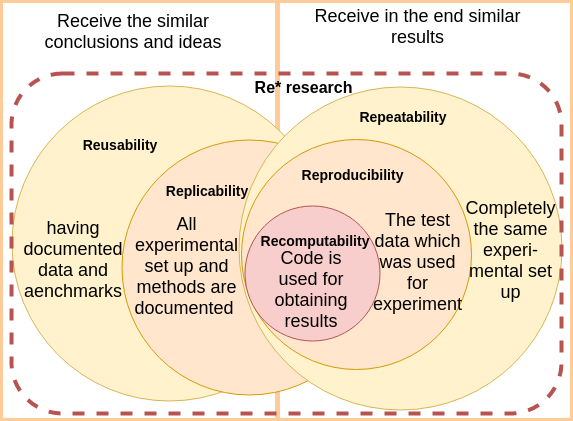
\includegraphics[scale=0.45]{fig/relationdiagram.png}
  \caption{Relation diagram}
  \label{fig:relationdiagram}
\end{figure}
As can be seen, two characteristics for which includes all other aims, concepts and satisfied criteria are Repeatability and Reusability.
\subsection{Good practices}
\begin{itemize}
    \item \textbf{Codebase.} computation-based experiments have the critical issue of having everything published and use as long as it possible only open source components. Everything should be documented and work out of the box. Using Docker image would be the good solution for this. Always leave links in the paper where the sources can be found.
    \item \textbf{Experimental set-up.} All hardware and software characteristics should be well described in the paper. For having similar software setup sharing the virtual machine image would solve most of the problems. It is more difficult for having the same hardware setup. To solve this problem all experiments can be done in a virtual machine, and the virtual machine image can be shared afterward. 
    \item \textbf{Experiments.}  Both datasets initial the same as result ones should be in open access. Also, all benchmarks and methods should be documented. 
    \item \textbf{Documentation.} Complete workflow, processes, and problems should be fully documented and provided together with the paper.
\end{itemize}
\subsection{Important workflows}
\begin{itemize}
    \item \textbf{Statistical methods.} Observable phenomena postulate hypotheses about and then measure. In system studies, the usual performance is the performance measured by the execution time. Some factors include many factors based on the architecture, operating system, compiler, and application. Some elements are controlled by the experimenter (i.e., architecture, compiler parameters or the time of the experiment). There are uncontrollable factors, some of which can be observed, and some of them can not. All independent elements should be randomized. Some parts of the experiment may be beyond the control of the experimenter. Real-time systems respond to real-world incentives, which are themselves random.
    \item \textbf{Documentation.} Proper archiving and documentation allow this even after a long time after the actual hardware or software infrastructure for repeating the experiment becomes unavailable. Indeed, this can also lead to negative results, such as the detection of errors in earlier experiments. The community must provide means of correcting published documents for these cases.
    \item \textbf{Benchmarks.} Experimental studies in systems are based on control applications. The test is a factor in the experiment, like everything else. When the experiment is started only in one of the stages, the value of interest is measured just for this test. If the standard is an application that the user wants to run, then this is normal (modulo). Otherwise, to make more general conclusions, the control factor should also be randomized: work with a variety of different criteria that are representative of real applications and statistically summarize the results.
\end{itemize}
\subsection{Software solutions}
There are plenty of solutions made to solve Re* research problem not only in computation-based works:
\begin{itemize}
    \item \textbf{PopperCI}\cite{DBLP:conf/infocom/JimenezAALMMR17}: Continuous Integration Service (CI), located in UC Santa Cruz, which allows researchers to automate end-to-end execution and verification of experiments. PopperCI suggests that tests follow Popper, a convention for implementing operations and writing articles after the DevOps approach, which recently proposed. PopperCI launches trials on cloud infrastructures with state, private or public funding in a fully automated way. 
    \item \textbf{ARTENOLIS}\cite{DBLP:journals/corr/abs-1712-05236}: The automated environment for reproducibility and testing for licensed software. The software is a universal software application for the infrastructure that implements continuous integration for open source software with licensed dependencies. It uses the master-slave structure, tests the code on several operating systems and several versions of the dependencies of the licensed software. ARTENOLIS provides stability, integrity and cross-platform compatibility of the codebase in the COBRA Toolbox and related tools.
    \item \textbf{ReproZip}\cite{DBLP:conf/sigmod/ChirigatiRSF16}: Computational reproducibility using Ease.ReproZip is the recommended packaging tool for reviewing the reproducibility of SIGMOD. ReproZip was designed to simplify the process of creating an actual computational experiment, reproduced on different platforms, even when the experiment combines without repeatability. The tool creates a stand-alone package for the experiment, automatically monitoring and determining all the dependencies it needs. The researcher can share the package with others.
    \item \textbf{COLIBRI}\cite{DBLP:conf/iccbr/Recio-GarciaDG13}: Studio, which supports researchers in creating Case-based Reasoning (CBR) systems through documented views with varying degrees of abstraction. These workflows - mandatory templates - can be passed on to the community to advance their future reference and reproducibility.
    \item \textbf{CARE}\cite{DBLP:conf/pldi/JaninVD14}: A comprehensive archiver for reproduced performance in Linux. CARE works in userland does not require configuration, and performs one task: creating an archive containing the selected executable files and files. To reproduce the final results of this initial launch is enough to unpack the archive, which has all the necessary tools for re-execution in a limited environment.
    \item \textbf{SUSHI}\cite{DBLP:journals/bmcbi/HatakeyamaORQSR16}: A defined workflow for a fully documented, reproducible and reusable analysis of NGS data. SUSHI is a flexible data analysis system that eliminates bioinformatics from the administrative problems of their data analysis. SUSHI allows users to create reproducible workflows of data analysis from individual applications and manage input data, parameters, meta information with user-controlled semantics, and work scripts. As distinctive features, SUSHI provides an expert command line interface, as well as a user-friendly web interface for launching bioinformatics tools. SUSHI datasets are self-contained and self-documented in the file system.
    \item \textbf{Dugong}\cite{DBLP:journals/bioinformatics/MenegidioJON18}: It is Docker image which based on Ubuntu Linux focused on the reproducibility and reproducibility for the analysis of bioinformatics. Image Docker is base on Ubuntu 16.04, which automates the installation of more than 3500 bioinformatics tools (along with their respective libraries and dependencies) in alternative computing environments. The software runs through the user-friendly graphical interface XFCE4, which allows the user to manage and install the Jupyter Notebook to help in the delivery and exchange of serial and reproducible protocols and results in the labs, improving in the development of open science projects.
    \item \textbf{S2P}\cite{DBLP:journals/cmpb/Lopez-Fernandez18}: A software tool for fast implementation of reproducible biomedical research projects. The software provides various functionalities for the process of identifying data based on 2D-gel proteins and MALDI-mass spectrometry with an automated reproduced manner.


\end{itemize}
\section{Conclusion}
Recently computation-based experiments start getting more and more complex regarding setup, processes, methods, and interactions. With growing complexity of tests, it has become more difficult to reproduce results from the author. Not reproducible results are not convenient in a scientific world that is why a concept of Re* research became so popular recently. Re*research consist of repeatability, reprehensibility, recomputability, reusability, and replicability. Most of the authors who were trying to solve this problem were generalizing it as term reproducibility, but in fact, they were always talking about Re research. \par
In this work, we have defined all of this characteristics separately with their definitions, features, current state of problems and recommendations. Also, we made a relational diagram where all of them were placed. The fact that research is repeatable and reusable typically mean that it satisfied all Re*research requirements. Most of the recommendations can be said in simple words document and upload everything. This problem is fundamental now and a lot of pieces software in different areas of research trying and solving most of the challenges. 

% The following two commands are all you need in the
% initial runs of your .tex file to
% produce the bibliography for the citations in your paper.
\bibliographystyle{abbrv}
\bibliography{vldb_sample}  % vldb_sample.bib is the name of the Bibliography in this case
% You must have a proper ".bib" file
%  and remember to run:
% latex bibtex latex latex
% to resolve all references




\end{document}
